% !TEX root = ../master.tex

\vspace*{.5cm}
\section{Goethe-Institut Porto Alegre}
\begin{center}
\emph{Rosa Helena Cunha Vidal}
\end{center}
\vspace*{1cm}

%body
\hypertarget{zeigen-sie-uns-den-ort-in-ihrer-bibliothek-an-dem-sie-die-meiste-zeit-verbringen.-was-ist-das-fuxfcr-ein-ort-wieso-sind-sie-die-meiste-zeit-dort}{%
\subsubsection*{Zeigen Sie uns den Ort in Ihrer Bibliothek, an dem Sie die
meiste Zeit verbringen. Was ist das für ein Ort? Wieso sind Sie die
meiste Zeit
dort?}\label{zeigen-sie-uns-den-ort-in-ihrer-bibliothek-an-dem-sie-die-meiste-zeit-verbringen.-was-ist-das-fuxfcr-ein-ort-wieso-sind-sie-die-meiste-zeit-dort}}

\begin{center}
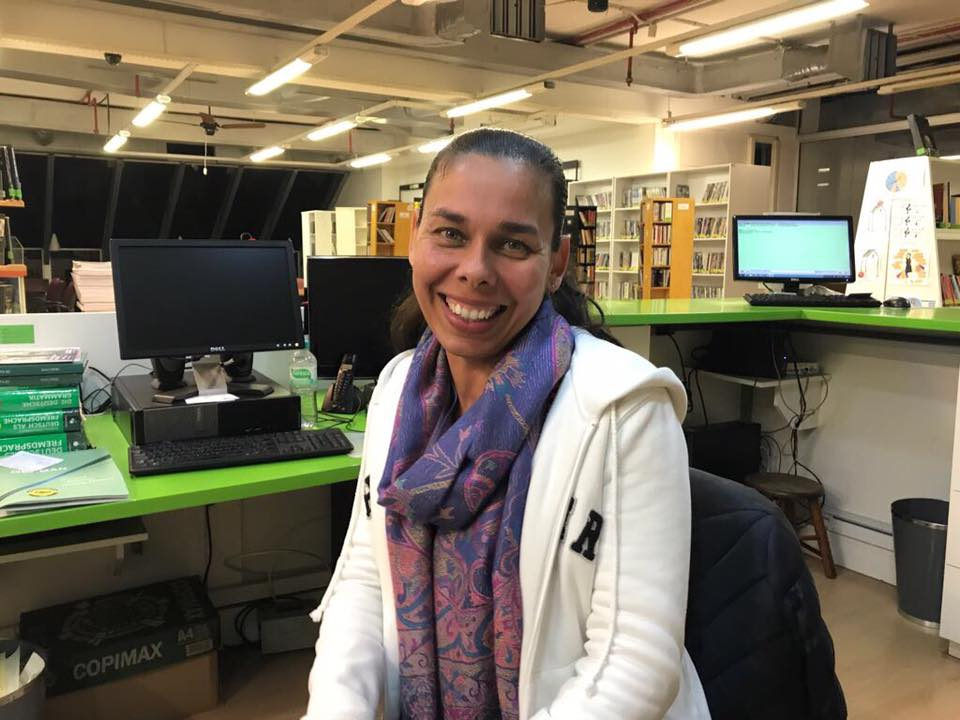
\includegraphics{gi-porto-alegre/img/onde-passo.jpg}
\end{center}

Der Ort ist die Bibliothek, wo ich den Kundendienst und die
Katalogisierung mache.

\hypertarget{was-wuxfcrden-sie-vermissen-wenn-es-nicht-mehr-da-wuxe4re-wieso-wuxfcrden-sie-es-vermissen}{%
\subsubsection*{Was würden Sie vermissen, wenn es nicht mehr da wäre? Wieso
würden Sie es
vermissen?}\label{was-wuxfcrden-sie-vermissen-wenn-es-nicht-mehr-da-wuxe4re-wieso-wuxfcrden-sie-es-vermissen}}

\begin{center}
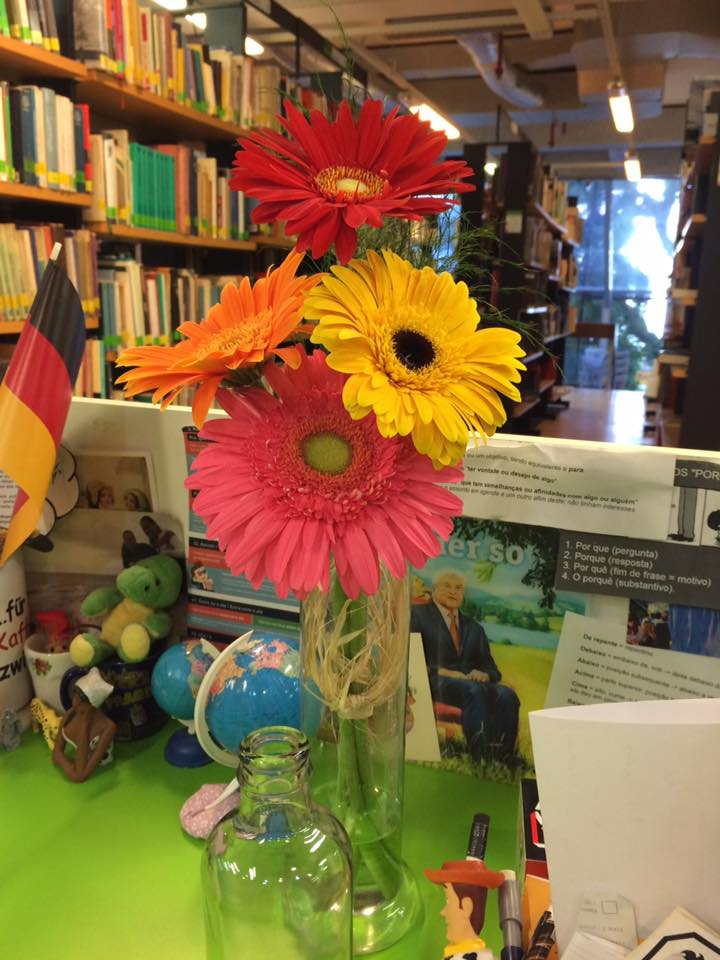
\includegraphics{gi-porto-alegre/img/meu-canto.jpg}
\end{center}

Weil ich die Bibliothek ein bisschen bin und die Bibliothek ist ein
bisschen von mir.

\hypertarget{was-stuxf6rt-sie-an-ihrer-bibliothek-beziehungsweise-was-wuxfcrden-sie-gerne-verbessern-wieso-stuxf6rt-sie-das-jetzt-noch}{%
\subsubsection*{Was stört Sie an Ihrer Bibliothek beziehungsweise was würden
Sie gerne verbessern? Wieso stört Sie das jetzt
(noch)?}\label{was-stuxf6rt-sie-an-ihrer-bibliothek-beziehungsweise-was-wuxfcrden-sie-gerne-verbessern-wieso-stuxf6rt-sie-das-jetzt-noch}}

\begin{center}
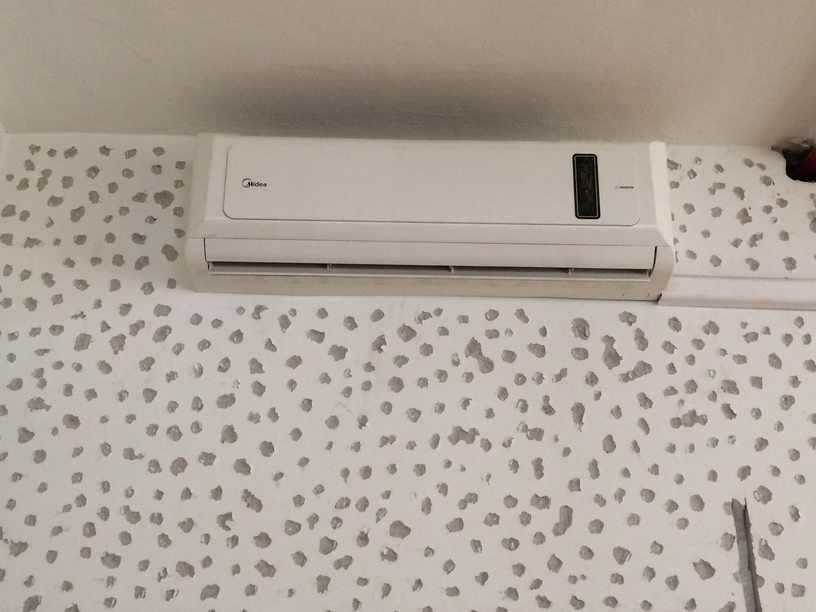
\includegraphics{gi-porto-alegre/img/ar.jpg}
\end{center}

Weil es wenige Klimaanlagen in der Bibliothek gibt und sie ist deshalb
im Sommer zu warm.

\hypertarget{zeigen-sie-uns-spuren-der-bibliotheksnutzung.-gibt-es-dazu-eine-geschichte}{%
\subsubsection*{Zeigen Sie uns Spuren der Bibliotheksnutzung. Gibt es dazu eine
Geschichte?}\label{zeigen-sie-uns-spuren-der-bibliotheksnutzung.-gibt-es-dazu-eine-geschichte}}

\begin{center}
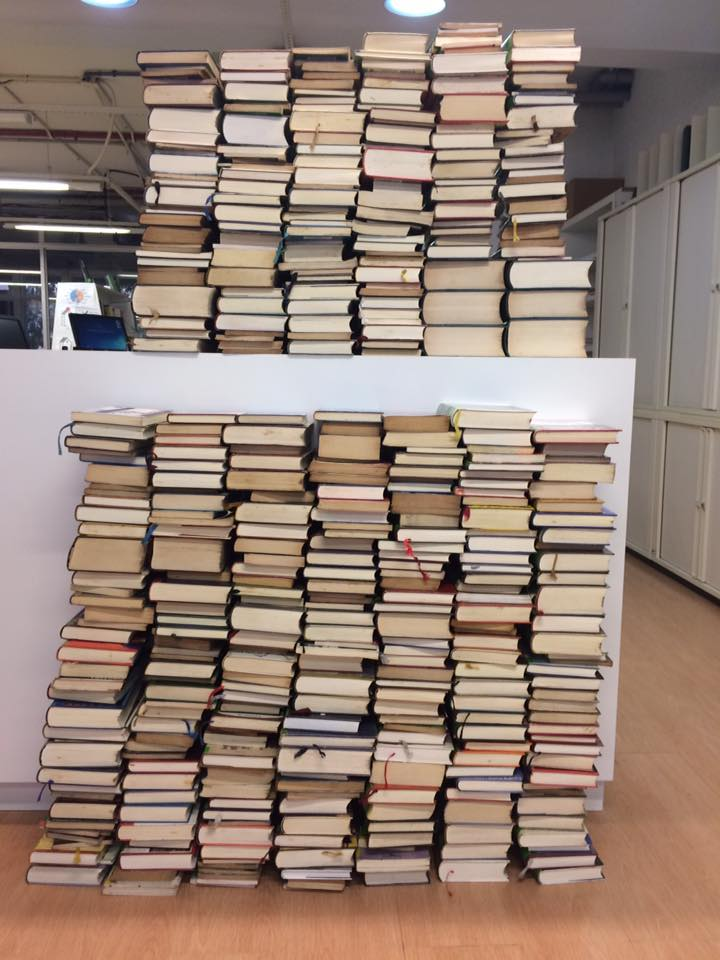
\includegraphics[width=0.4\textwidth]{gi-porto-alegre/img/descarte.jpg}
\end{center}

Bücher aussondern.

\hypertarget{was-haben-sie-was-die-anderen-nicht-haben-warum-haben-sie-das-sollten-andere-es-auch-in-ihren-bibliotheken-haben}{%
\subsubsection*{Was haben Sie, was die anderen nicht haben? Warum haben Sie
das? Sollten andere es auch in ihren Bibliotheken
haben?}\label{was-haben-sie-was-die-anderen-nicht-haben-warum-haben-sie-das-sollten-andere-es-auch-in-ihren-bibliotheken-haben}}

\begin{center}
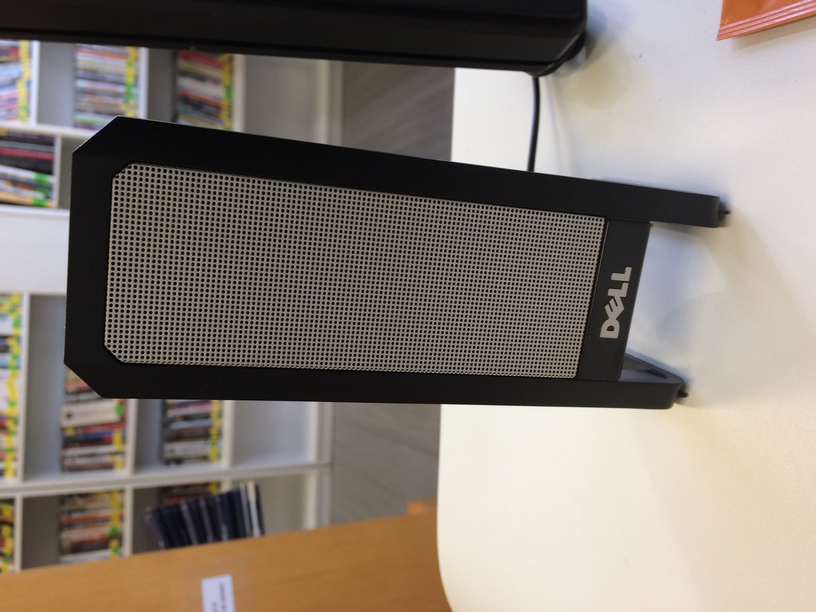
\includegraphics{gi-porto-alegre/img/musica.jpg}
\end{center}

Musik. Bibliothek sollen auch Hintergrundmusik haben.

\hypertarget{ihre-bibliothek-name-adresse-spezialisierung-was-man-noch-uxfcber-sie-wissen-sollte}{%
\subsubsection*{Ihre Bibliothek (Name, Adresse, Spezialisierung, was man noch
über sie wissen
sollte)?}\label{ihre-bibliothek-name-adresse-spezialisierung-was-man-noch-uxfcber-sie-wissen-sollte}}

Goethe-Institut Porto Alegre -- Bibliothek. Rua 24 de Outubro, 112,
Porto Alegre, RS -- Brasil CEP 90510-000

%autor
\begin{center}\rule{0.5\linewidth}{\linethickness}\end{center}

\textbf{Rosa Helena Cunha Vidal}, Bibliothekarin.
